\documentclass[border=10pt]{standalone}
\usepackage{tikz}
\usetikzlibrary{positioning, arrows.meta, calc}
\usepackage{amsmath, amssymb}

\begin{document}
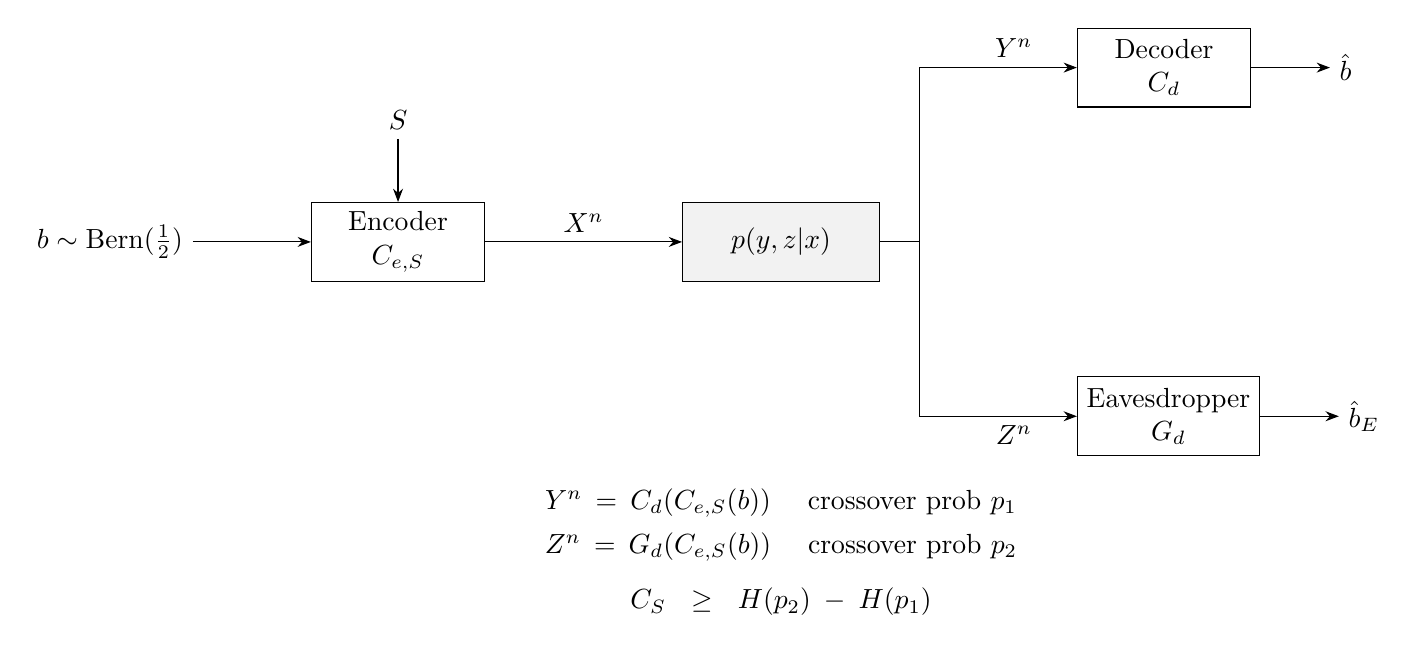
\begin{tikzpicture}[
    >=Stealth,
    node distance=1.8cm,
    block/.style={draw, rectangle, minimum width=2.2cm, minimum height=1cm, align=center},
    channel/.style={draw, rectangle, minimum width=2.5cm, minimum height=1cm, align=center, fill=gray!10},
    every edge/.style={draw, ->},
]

% Encoder
\node[block] (enc) {Encoder\\$C_{e,S}$};

% Channel
\node[channel, right=2.5cm of enc] (ch) {$p(y,z|x)$};

% Bob decoder
\node[block, above right=1.2cm and 2.5cm of ch] (bob) {Decoder\\$C_d$};

% Eve decoder
\node[block, below right=1.2cm and 2.5cm of ch] (eve) {Eavesdropper\\$G_d$};

% Input/output labels
\node[left=1.5cm of enc] (msg) {$b \sim \text{Bern}(\tfrac{1}{2})$};
\node[right=1cm of bob] (bhat) {$\hat{b}$};
\node[right=1cm of eve] (beve) {$\hat{b}_E$};

% Sentence input
\node[above=0.8cm of enc] (sent) {$S$};

% Arrows
\draw[->] (msg) -- (enc);
\draw[->] (sent) -- (enc);
\draw[->] (enc) -- node[above] {$X^n$} (ch);
\draw[->] (ch.east) -- ++(0.5,0) |- node[above, pos=0.8] {$Y^n$} (bob.west);
\draw[->] (ch.east) -- ++(0.5,0) |- node[below, pos=0.8] {$Z^n$} (eve.west);
\draw[->] (bob) -- (bhat);
\draw[->] (eve) -- (beve);

% Channel details - BSC parameters
\node[below=2.5cm of ch, align=center, text width=7cm] (info) {
    $Y^n = C_d(C_{e,S}(b))$ \quad crossover prob $p_1$\\[4pt]
    $Z^n = G_d(C_{e,S}(b))$ \quad crossover prob $p_2$\\[8pt]
    $C_S \geq H(p_2) - H(p_1)$
};

\end{tikzpicture}
\end{document}
